%%%%%%%%%%%%%%%%%%%%%%%%%%%%%%%%%%%%%%%%%
% HW Template
% LaTeX Template
% Version 1.0 (19/10/18)
% Modified by
% Erdem TUNA
% Halil TEMURTAŞ 
% Enes TAŞTAN 
%%%%%%%%%%%%%%%%%%%%%%%%%%%%%%%%%%%%%%%%%
%
%----------------------------------------------------------------------------------------
%	PACKAGES AND OTHER DOCUMENT CONFIGURATIONS
%----------------------------------------------------------------------------------------
\documentclass[a4paper,12pt]{article}
%-----packages------
\usepackage[a4paper, total={6.5in, 8.5in}]{geometry}
\usepackage[english]{babel}
\usepackage[utf8x]{inputenc}
\usepackage{amsmath}
\usepackage{graphicx}
\usepackage[colorinlistoftodos]{todonotes}
\usepackage{gensymb} % this could be problem
\usepackage{float}
\usepackage{fancyref}
\usepackage{subcaption}
\usepackage[toc,page]{appendix} %appendix package
\usepackage{xcolor}
\usepackage{listings}
\usepackage{xspace}
\usepackage{amssymb}
\usepackage{nicefrac}
\usepackage{gensymb}
\usepackage{fancyhdr}
\usepackage{blindtext}  % for dummy text, use \blindtext or \BlindText
\usepackage[final]{pdfpages}  % pdf include
\usepackage{array} %allows more options in tables
\usepackage{pgfplots,pgf,tikz} %coding plots in latex
\usepackage{capt-of} % allows caption outside the figure environment
\usepackage[export]{adjustbox} %more options for adjusting the images
\usepackage{multicol,multirow,slashbox} % allows tables like table1
%\usepackage[hyperfootnotes=false]{hyperref} % clickable references
\usepackage{epstopdf} % useful when matlab is involved
%\usepackage{placeins} % prevents the text after figure to go above figure with \FloatBarrier 
%\usepackage{listingsutf8,mcode} %import .m or any other code file mcode is for matlab highlighting

%-----end of packages

%-----specifications-----
\definecolor{mGreen}{rgb}{0,0.6,0} % for python
\definecolor{mGray}{rgb}{0.5,0.5,0.5}
\definecolor{mPurple}{rgb}{0.58,0,0.82}
\definecolor{mygreen}{RGB}{28,172,0} % color values Red, Green, Blue for matlab
\definecolor{mylilas}{RGB}{170,55,241}

\setcounter{secnumdepth}{5} % how many sectioning levels to assign numbers to
\setcounter{tocdepth}{5}    % how many sectioning levels to show in ToC

\lstdefinestyle{CStyle}{
	commentstyle=\color{mGreen},
	keywordstyle=\color{magenta},
	numberstyle=\tiny\color{mGray},
	stringstyle=\color{mPurple},
	basicstyle=\footnotesize,
	breakatwhitespace=false,         
	breaklines=true,
	frame=single,
	rulecolor=\color{black!40},                 
	captionpos=b,                    
	keepspaces=true,                 
	numbers=left,                    
	numbersep=5pt,                  
	showspaces=false,                
	showstringspaces=false,
	showtabs=false,                  
	tabsize=2,
	language=C
}

\lstset{language=Matlab,%
	%basicstyle=\color{red},
	breaklines=true,%
	frame=single,
	rulecolor=\color{black!40},
	morekeywords={matlab2tikz},
	keywordstyle=\color{blue},%
	morekeywords=[2]{1}, keywordstyle=[2]{\color{black}},
	identifierstyle=\color{black},%
	stringstyle=\color{mylilas},
	commentstyle=\color{mygreen},%
	showstringspaces=false,%without this there will be a symbol in the places where there is a space
	numbers=left,%
	numberstyle={\tiny \color{black}},% size of the numbers
	numbersep=9pt, % this defines how far the numbers are from the text
	emph=[1]{for,end,break},emphstyle=[1]\color{red}, %some words to emphasise
	%emph=[2]{word1,word2}, emphstyle=[2]{style},    
}


\tikzset{
	desicion/.style={
		diamond,
		draw,
		text width=4em,
		text badly centered,
		inner sep=0pt
	},
	block/.style={
		rectangle,
		draw,
		text width=10em,
		text centered,
		rounded corners
	},
	cloud/.style={
		draw,
		ellipse,
		minimum height=2em
	},
	descr/.style={
		fill=white,
		inner sep=2.5pt
	},
	connector/.style={
		-latex,
		font=\scriptsize
	},
	rectangle connector/.style={
		connector,
		to path={(\tikztostart) -- ++(#1,0pt) \tikztonodes |- (\tikztotarget) },
		pos=0.5
	},
	rectangle connector/.default=-2cm,
	straight connector/.style={
		connector,
		to path=--(\tikztotarget) \tikztonodes
	}
}

\tikzset{
	desicion/.style={
		diamond,
		draw,
		text width=4em,
		text badly centered,
		inner sep=0pt
	},
	block/.style={
		rectangle,
		draw,
		text width=10em,
		text centered,
		rounded corners
	},
	cloud/.style={
		draw,
		ellipse,
		minimum height=2em
	},
	descr/.style={
		fill=white,
		inner sep=2.5pt
	},
	connector/.style={
		-latex,
		font=\scriptsize
	},
	rectangle connector/.style={
		connector,
		to path={(\tikztostart) -- ++(#1,0pt) \tikztonodes |- (\tikztotarget) },
		pos=0.5
	},
	rectangle connector/.default=-2cm,
	straight connector/.style={
		connector,
		to path=--(\tikztotarget) \tikztonodes
	}
}
%-----end of specifications-----


%----commands----
\newcommand\nd{\textsuperscript{nd}\xspace}
\newcommand\rd{\textsuperscript{rd}\xspace}
\newcommand\nth{\textsuperscript{th}\xspace} %\th is taken already
\newcommand{\specialcell}[2][c]{ \begin{tabular}[#1]{@{}c@{}}#2\end{tabular}} % for too long table lines

\newcommand{\blankpage}{
	\- \\[9cm]	
	{ \centering \textit{This page intentionally left blank.} \par }
	\- \\[9cm]
}% For Blank Page

\makeatletter
\renewcommand\paragraph{\@startsection{paragraph}{4}{\z@}%
	{-2.5ex\@plus -1ex \@minus -.25ex}%
	{1.25ex \@plus .25ex}%
	{\normalfont\normalsize\bfseries}}
\makeatother
%-----end of commands-----


\pagestyle{fancy}
\fancyhead[LO,LE]{Halil TEMURTAŞ / 2094522 \\ İclal SATICI / 2094407 }
\fancyhead[RO,RE]{\today}
%\fancyfoot[RO,RE]{\includegraphics[width=2.7cm]{../../../Documents/Logo/logo}}

\begin{document}
\begin{center}
	\textbf{\large EE407 Process Control \\[0.2cm] HW 1} \\
\end{center}

\begin{enumerate}
	\item We will analyse the system shown in the \textit{Figure~\ref{fig:1a}}. 

		\begin{enumerate}
			\item To write the SS model of the system, let us begin with writing fundamental equation describing the system.
			
			$$	F_{Net}~=~m\ddot{x}~=~F-b\dot{x}-kx	$$
			
			Choosing x = ${[x~~\dot{x}]}^T$ and $ y = [1~~0] $x, we can build our Space-State Model for the system as 
			$$ \dot{x}~=~Ax+Bu  ~~ \& ~~  y~=~Cx+Du			$$
			
			\[
			\begin{bmatrix}
   				\dot{x} \\
   			 	\ddot{x}
			\end{bmatrix}
			=
			\begin{bmatrix}
    			0 & 1 \\
    			-k/m & -b/m
			\end{bmatrix}			
			\begin{bmatrix}
   				c \\
   			 	\dot{x}
			\end{bmatrix}
			+
			\begin{bmatrix}
   				0 \\
   			 	1/m
			\end{bmatrix}
			u
			\]
			
			where u is the input force F.
			
				\begin{figure}[H]
					\center
					\setlength{\unitlength}{\textwidth} 
					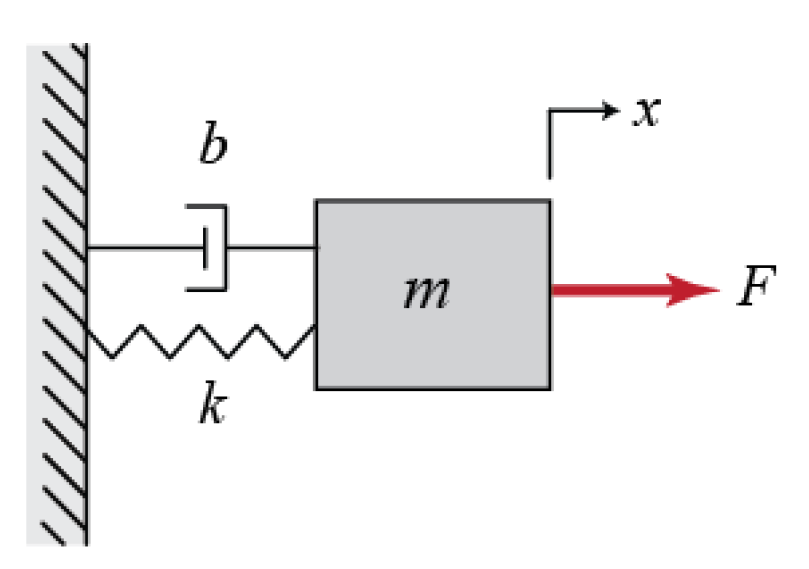
\includegraphics[width=0.4\unitlength]{images/1a}
					\caption{\label{fig:1a} Mass Spring Damper System }
				\end{figure}
			\item 	Simulink Model for the Mass Spring Damper System can be seen at \textit{Figure~\ref{fig:1b}}
				\begin{figure}[H]
					\center
					\setlength{\unitlength}{\textwidth} 
					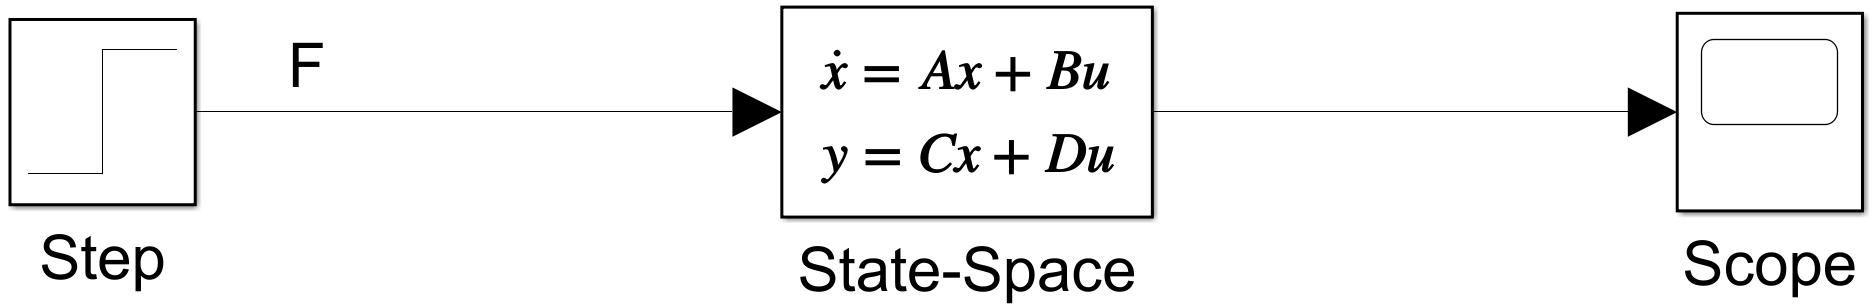
\includegraphics[width=0.9\unitlength]{images/1b}
					\caption{\label{fig:1b} Simulink Model for the Mass Spring Damper System }
				\end{figure}	\-\\		
			
			\item 	For the following subsections, the simulations are for the model when the applied force is a unit step function starting at t = 5 sec, i.e., $u(t-5)$.
			
				\begin{figure}[h]
					\center
					\setlength{\unitlength}{\textwidth} 
					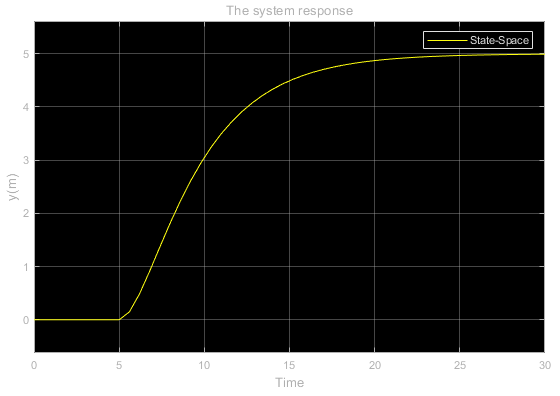
\includegraphics[width=0.8\unitlength]{images/1cy}
					\caption{\label{fig:1c} The System Response for MSD as m = 1kg, b = 0.2Ns/m, k = 1N/m }
				\end{figure}
			
				\begin{enumerate}
					\item The spring force is proportional to the displacement of the mass,x with the direction of opposite to the F. Therefore, when the spring constant decreased, the displacement of x is increased. The figures are consistent with these, \textit{Figure~\ref{fig:1c1}} has small k value and it reaches far than \textit{Figure~\ref{fig:1c}}.		
			
			\begin{figure}[h]
				\center
				\setlength{\unitlength}{\textwidth} 
				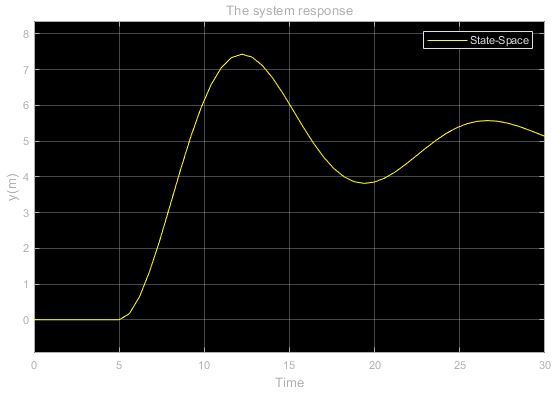
\includegraphics[width=0.8\unitlength]{images/1c1y}
				\caption{\label{fig:1c1} The System Response for MSD as m = 1kg, b = 0.2Ns/m, k = 0.2N/m }
			\end{figure}
			
			
			
			\item It is known that $F_{net}=ma=m\ddot{x} $ , then mass and acceleration that is related to position are oppositely proportional, so when mass increased, the output will be decreased. The \textit{Figure~\ref{fig:1c}} and \textit{Figure~\ref{fig:1c2}} are expected.
			
			\begin{figure}[H]
				\center
				\setlength{\unitlength}{\textwidth} 
				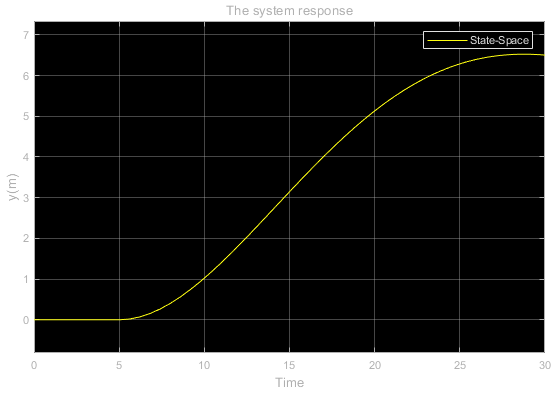
\includegraphics[width=0.8\unitlength]{images/1c2y}
				\caption{\label{fig:1c2} The System Response for MSD as m = 10kg, b = 0.2Ns/m, k = 1N/m }
			\end{figure}
			
			\item  The viscous damping force is proportional to the velocity of the mass, $v=\dot{x}$ with the direction of opposite to the F. In this case, firstly this opposite direction is not so much because of the velocity is small and after some point this velocity value increases and effect the system with more opposite force. Therefore, \textit{Figure~\ref{fig:1c}} and \textit{Figure~\ref{fig:1c3}} are expected.
			
			\begin{figure}[H]
				\center
				\setlength{\unitlength}{\textwidth} 
				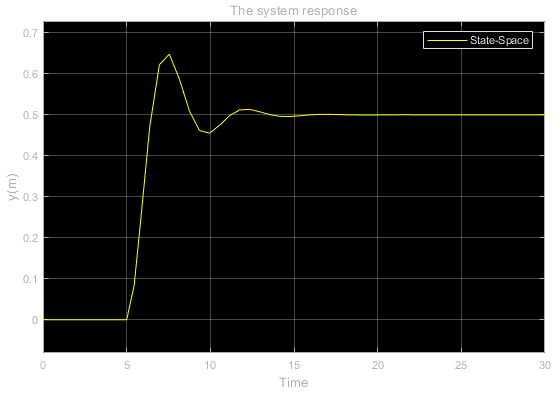
\includegraphics[width=0.8\unitlength]{images/1c3y}
				\caption{\label{fig:1c3} The System Response for MSD as m = 1kg, b = 2Ns/m, k = 1N/m }
			\end{figure}	
			
		\end{enumerate}			
			
			\item 	d
				\begin{figure}[H]
					\center
					\setlength{\unitlength}{\textwidth} 
					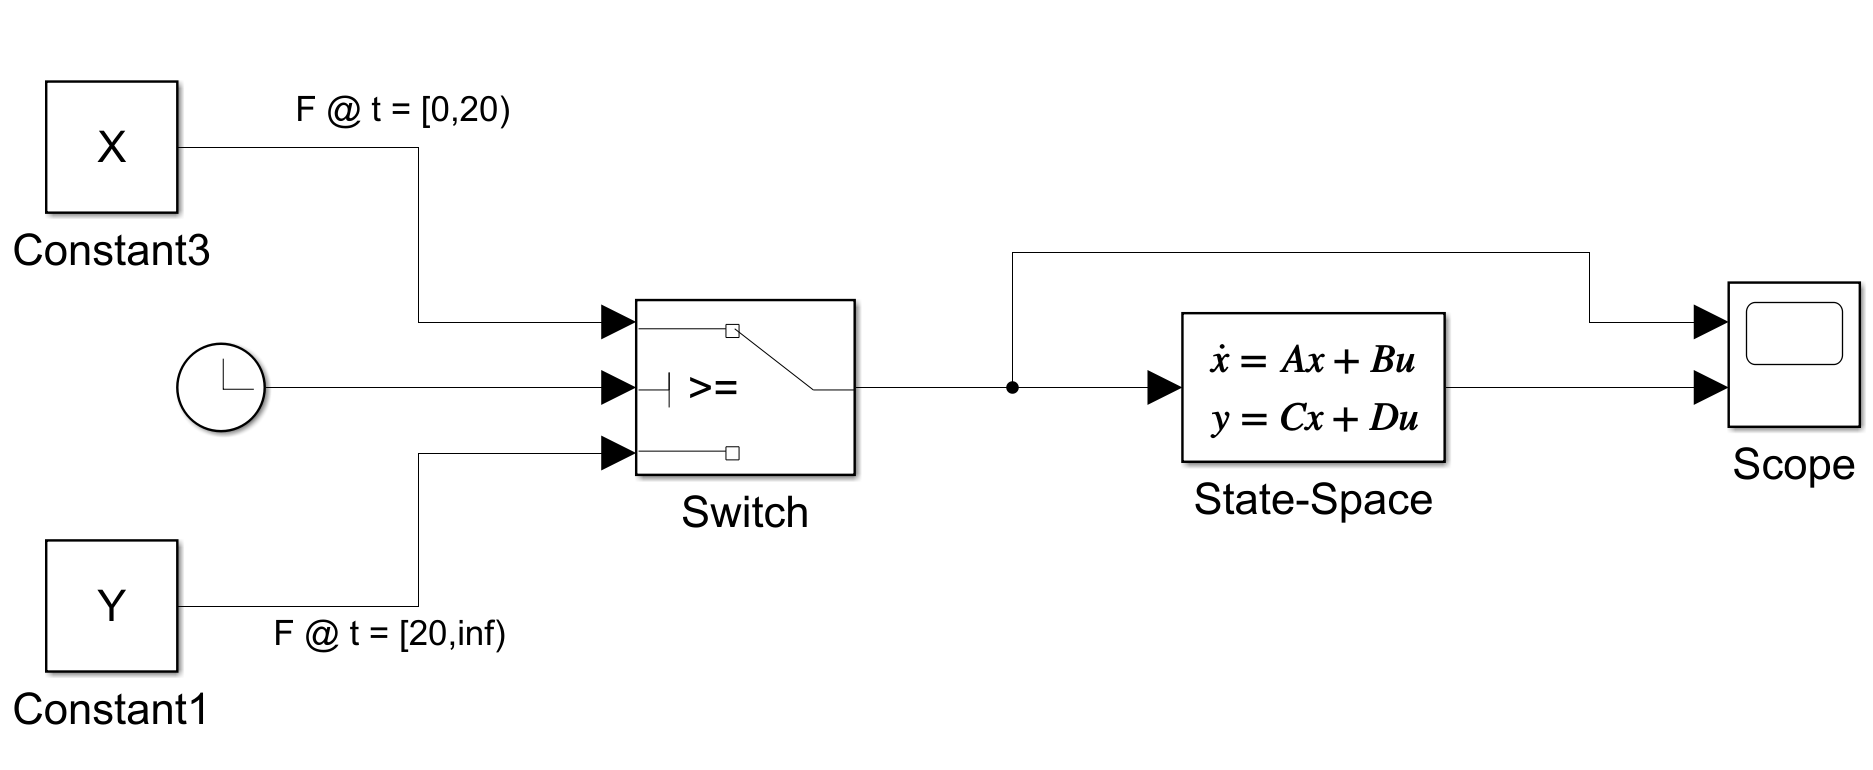
\includegraphics[width=0.8\unitlength]{images/1d1}
					\caption{\label{fig:1d1} Simulink Model for the MSD with Varying Input Force }
				\end{figure}
				
				\begin{figure}[H]
					\center
					\setlength{\unitlength}{\textwidth} 
					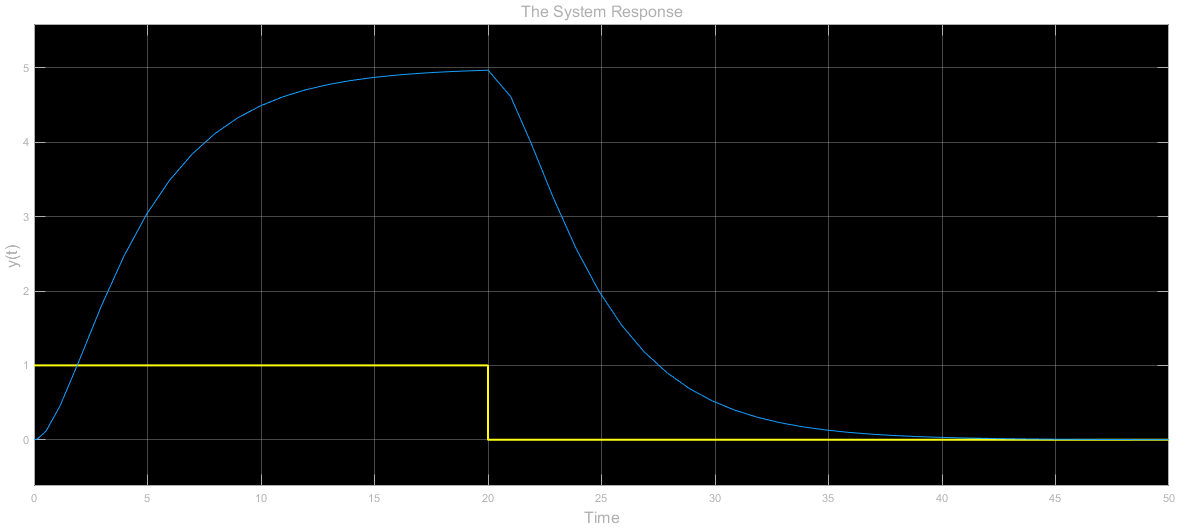
\includegraphics[width=0.8\unitlength]{images/1d2}
					\caption{\label{fig:1d2} The System Response for MSD as the Input Changes at t=20 s }
				\end{figure}
				
			\item 	e
				
				
				
			
			
			\item 	f
			
				\begin{figure}[H]
					\center
					\setlength{\unitlength}{\textwidth} 
					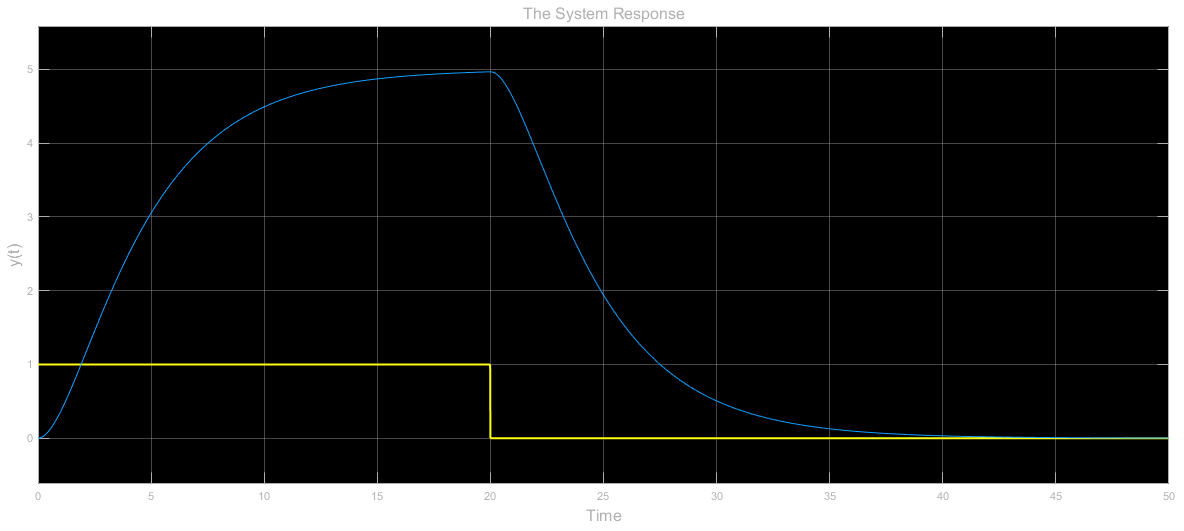
\includegraphics[width=0.8\unitlength]{images/1f}
					\caption{\label{fig:1f} The System Response for MSD with Desired Parameters in Q1f  }
				\end{figure}
				
				\begin{figure}[H]
					\setlength{\unitlength}{\textwidth} 
					\centering
					\begin{subfigure}{.5\textwidth}
  						\centering
  						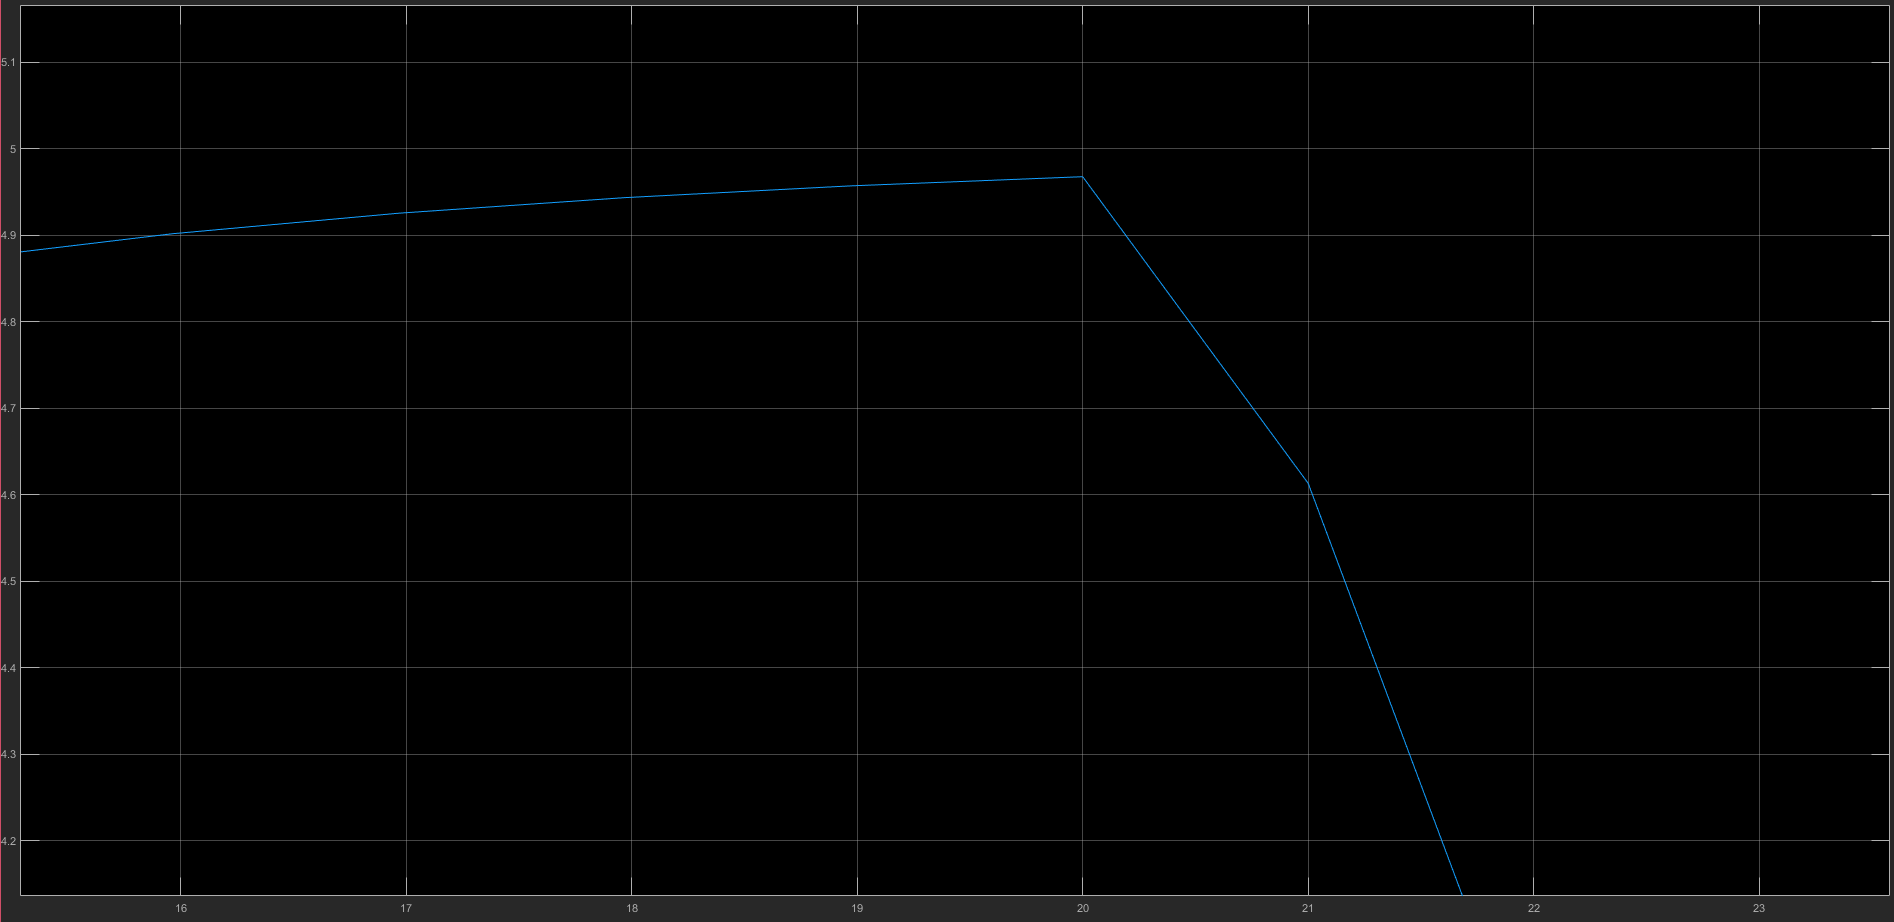
\includegraphics[width=0.48\unitlength]{images/1d22}
  						\caption{\label{fig:vary} Simulation with Variable Step }
					\end{subfigure}%
					\begin{subfigure}{.5\textwidth}
  						\centering
						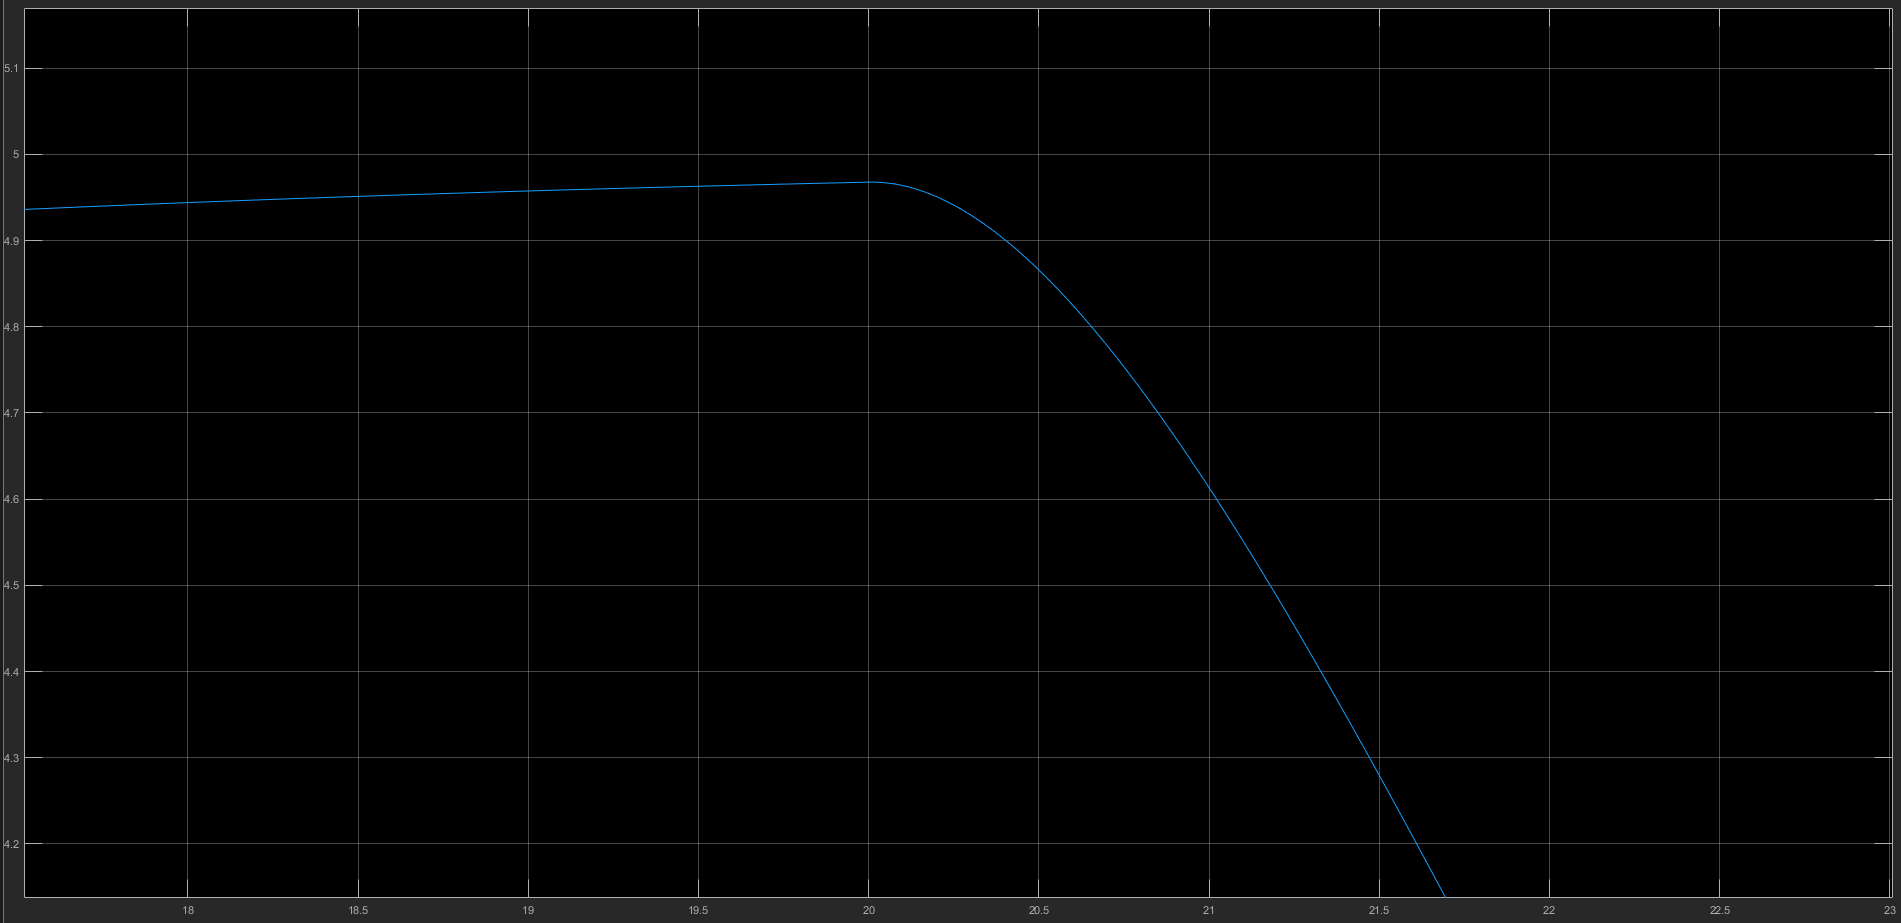
\includegraphics[width=0.48\unitlength]{images/1f2}
  						\caption{\label{fig:fixed} Simulation with Fixed Step}
					\end{subfigure}
					\caption{\label{fig:calisandegree} Simulation with Variable and Fixed Step   }
				\end{figure}
				
		\end{enumerate}
	
	
	\item 2. soru
		\begin{enumerate}
			\item a
			\item b
			\item c	
			\item d
		\end{enumerate}
		
		
		
		
		
		
\end{enumerate}
	
	
	
	
\end{document}

%----samples------
%\begin{itemize}
%\item Item
%\item Item
%\end{itemize}

%\begin{figure}[H]
%\center
%\setlength{\unitlength}{\textwidth} 
%\includegraphics[width=0.7\unitlength]{images/logo1}
%\caption{\label{fig:logo}Logo }
%\end{figure}

%\begin{figure}[H]
%	\setlength{\unitlength}{\textwidth} 
%	\centering
%	\begin{subfigure}{.5\textwidth}
%  		\centering
%  		\includegraphics[width=0.48\unitlength]{images/logo1}
%  		\caption{\label{fig:logo1}Logo1 }
%	\end{subfigure}%
%	\begin{subfigure}{.5\textwidth}
%  		\centering
%		\includegraphics[width=0.48\unitlength]{images/logo2}
%  		\caption{\label{fig:logo2}Logo2}
%	\end{subfigure}
%\caption{\label{fig:calisandegree} Small Logos   }
%\end{figure}
	
%\begin{table}[H]
%  \centering
% 
%    \begin{tabular}{c|c|c}
%       $$A$$ & $$B$$ & $$C$$ \\ \hline
%       1 & 2 & 3  \\ \hline
%       2 & 3 & 4  \\ \hline
%       3 & 4 & 5  \\ \hline
%       4 & 5 & 6  
%      
%  \end{tabular}
%  \caption{table}
%  \label{tab:table}
%\end{table}
	
%\begin{table}[H]
%  \centering
% 
%    \begin{tabular}{c|c|c}
%       \backslashbox{$A$}{$a$} & $$\specialcell{ Average deviation \\ after subtracting out the  \\ frequency error }$$ & $$C$$ \\ \hline
%       \multirow{2}{*}{1} & 2 & 3  \\ \cline{2-3}
%        & 3 & 4  \\ \hline
%       3 & \multicolumn{2}{c}{4}  \\ \hline
%       4 & 5 & 6  
%      
%  \end{tabular}
%  \caption{table}
%  \label{tab:table}
%\end{table}
%-----end of samples-----